\documentclass[crop,tikz]{standalone}
\usepackage{tikz}
\usepackage{amsmath,amssymb}

\definecolor{brewer1}{rgb}{0.105882,0.619608,0.466667}
\definecolor{brewer2}{rgb}{0.85098,0.372549,0.00784314}
\definecolor{brewer3}{rgb}{0.458824,0.439216,0.701961}
\definecolor{brewer4}{rgb}{0.905882,0.160784,0.541176}

\usetikzlibrary{arrows.meta, shapes, positioning, calc}

\tikzset{
  root/.style={rectangle, rounded corners, minimum width=2cm, minimum height=0.8cm, text centered, draw=black, fill=brewer2, line width=1pt},
  internalnode/.style={rectangle, minimum width=1.7cm, minimum height=0.7cm, text centered, draw=black, fill=gray!2},
  decision/.style={ellipse, minimum width=1.7cm, minimum height=0.7cm, text centered, draw=black, fill=gray!2},
  rpfunique/.style={rectangle, minimum width=1.7cm, minimum height=0.7cm, text centered, draw=black, fill=brewer1},
  rpfuniquedecision/.style={ellipse, minimum width=1.7cm, minimum height=0.7cm, text centered, draw=black, fill=brewer1},
  interaction/.style={rectangle, minimum width=1.7cm, minimum height=0.7cm, text centered, draw=black, fill=brewer3},
  arrow/.style={thick,->,>=stealth},
  label/.style={font=\scriptsize}
}


\begin{document}

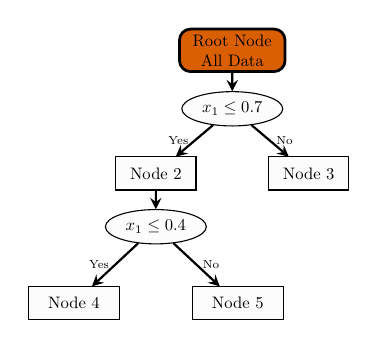
\begin{tikzpicture}[node distance=0.8cm and 1.1cm, scale=0.6, transform shape]

  % Root node
  \node (root) [root, text width=2cm, align=center] {Root Node\\All Data};

  % First level splits
  \node (b) [decision, below=0.4cm and 0.3cm of root] {$x_1 \leq 0.7$};

  % Connections from root
  \draw [arrow] (root) -- (b);
  % \draw [arrow] (root) -- (e);

  % % Nodes from first x1 split
  \node (c) [internalnode, below left=0.75cm and 0cm of b, text width=1.2cm, align=center] {Node 2};
  \node (d) [internalnode, below right=0.75cm and 0cm of b, text width=1.2cm, align=center] {Node 3};

  % % Connections from first split
  \draw [arrow] (b) -- node[label, left] {Yes} (c);
  \draw [arrow] (b) -- node[label, right] {No} (d);

  % % Further splits from Node 2
  \node (h) [decision, below=0.4cm and 0cm of c] {$x_1 \leq 0.4$};
  % \node (k) [rpfunique, below right=1.2cm and 0cm of c] {$x_3 \leq 0.3$};

  % % Connections from Node 2
  \draw [arrow] (c) -- (h);
  % \draw [arrow] (c) -- (k);

  % % Nodes from x1 <= 0.4 split
  \node (i) [internalnode, below left=1cm and 0cm of h, text width=1.7cm, align=center] {Node 4};
  \node (j) [internalnode, below right=1cm and 0cm of h, text width=1.7cm, align=center] {Node 5};

  % Connections from x1 <= 0.4 split
  \draw [arrow] (h) -- node[label, left] {Yes} (i);
  \draw [arrow] (h) -- node[label, right] {No} (j);
\end{tikzpicture}
\end{document}
